%
% ritzkoef.tex -- Refraktion mit Ritz
%
% (c) 2021 Prof Dr Andreas Müller, OST Ostschweizer Fachhochschule
%
\bgroup
\begin{frame}[t]
\setlength{\abovedisplayskip}{5pt}
\setlength{\belowdisplayskip}{5pt}
\frametitle{Refraktion: Konvergenz}
\begin{center}
\begin{tikzpicture}[>=latex,thick]
\node at (0,0) {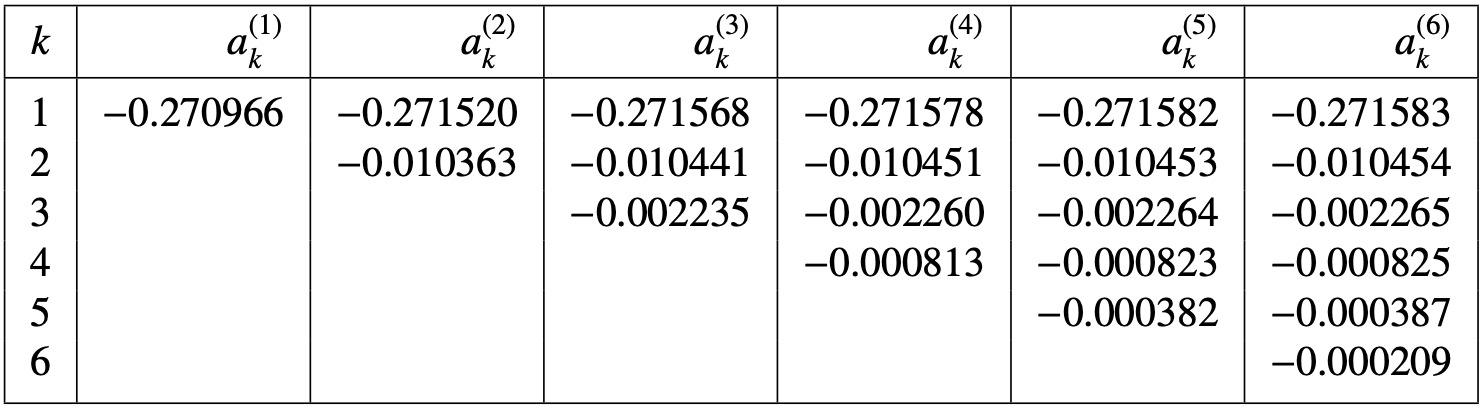
\includegraphics[width=\textwidth]{../slides/6/ritzloesung.png}};
\end{tikzpicture}
\end{center}
\end{frame}
\egroup
